\documentclass[border={10pt, 10pt, 10pt, 10pt}]{standalone}

\usepackage{tikz}
\usepackage{graphicx}
\usepackage{varwidth}

\renewcommand\familydefault{\sfdefault}

\begin{document}
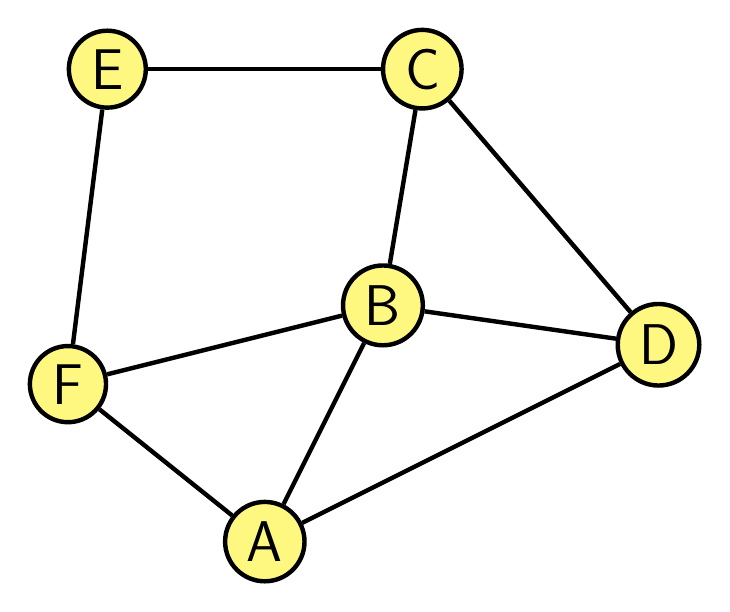
\begin{tikzpicture}

\node[draw=black, fill=yellow!50, circle, ultra thick] (A) at (0, 0) {\huge A};
\node[draw=black, fill=yellow!50, circle, ultra thick] (B) at (1.5, 3) {\huge B};
\node[draw=black, fill=yellow!50, circle, ultra thick] (C) at (2, 6) {\huge C};
\node[draw=black, fill=yellow!50, circle, ultra thick] (D) at (5, 2.5) {\huge D};
\node[draw=black, fill=yellow!50, circle, ultra thick] (E) at (-2, 6) {\huge E};
\node[draw=black, fill=yellow!50, circle, ultra thick] (F) at (-2.5, 2) {\huge F};

\draw[ultra thick] (A) -- (F);
\draw[ultra thick] (A) -- (B);
\draw[ultra thick] (C) -- (B);
\draw[ultra thick] (C) -- (D);
\draw[ultra thick] (B) -- (D);
\draw[ultra thick] (E) -- (F);
\draw[ultra thick] (E) -- (C);
\draw[ultra thick] (B) -- (F);
\draw[ultra thick] (A) -- (D);

\end{tikzpicture}
\end{document}